% Data flow diagram
% Template adapted from http://www.texample.net/tikz/examples/data-flow-diagram/ by David Fokkema
\documentclass{article}
\usepackage{tikz}
\usetikzlibrary{arrows,shapes}

% Custom, should be provided in the same directory.
\usepackage{datastore}

\begin{document}
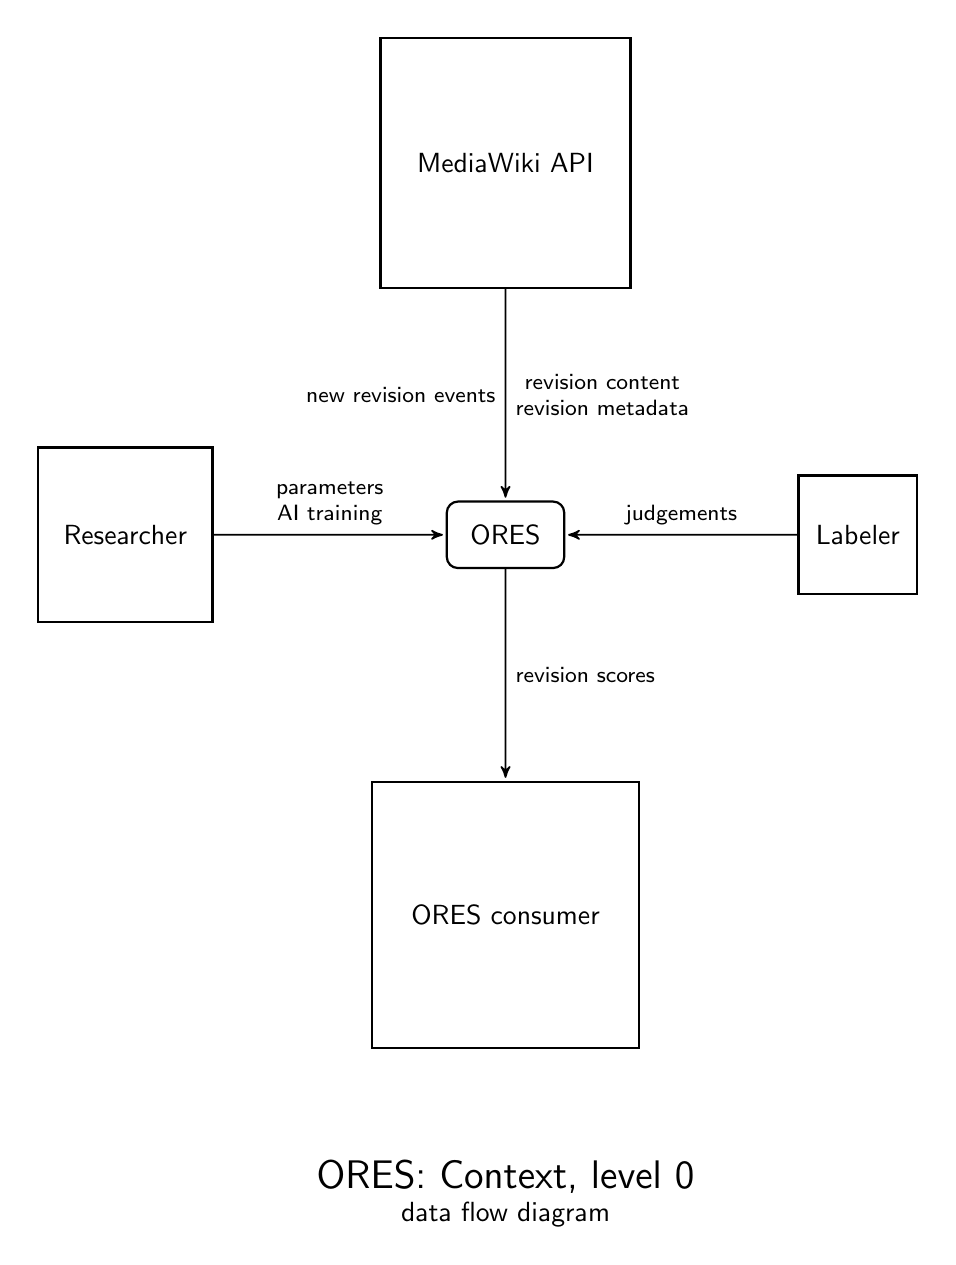
\begin{tikzpicture}[
  font=\sffamily,
  every matrix/.style={ampersand replacement=\&,column sep=2cm,row sep=2cm},
  interface/.style={draw,thick,regular polygon,regular polygon sides=4,inner sep=0},
  process/.style={draw,thick,rounded corners,inner sep=.3 cm},
  datastore/.style={draw,thick,shape=datastore,inner sep=.3cm},
  to/.style={->,>=stealth',shorten >=1pt,semithick,font=\sffamily\footnotesize},
  every node/.style={align=center}]

  % Position the nodes using a matrix layout
  \matrix{
      \& \node[interface] (mwapi) {MediaWiki API}; \\
    \node[interface] (researcher) {Researcher};
      \& \node[process] (ores) {ORES};
        \& \node[interface] (labeler) {Labeler}; \\
      \& \node[interface] (consumer) {ORES consumer}; \\
  };

  \node [below=3cm, align=flush center] at (consumer)
  {\Large ORES: Context, level 0 \\ \normalsize data flow diagram};

  % Draw the arrows between the nodes and label them.
  \draw[to] (mwapi) -- node[midway,left] {new revision events}
      node[midway,right] {revision content \\ revision metadata} (ores);
  \draw[to] (ores) -- node[midway,right] {revision scores} (consumer);
  \draw[to] (researcher) -- node[midway,above] {parameters \\ AI training} (ores);
  \draw[to] (labeler) -- node[midway,above] {judgements} (ores);
\end{tikzpicture}
\end{document}
